\section{BON extraction}
In section \ref{design-bon-extraction} it was mentioned that the textual \textsc{bon} extraction tool consists of two parts, the interface to the EIffel world and an internal representation of textual \textsc{bon}. This section will describe the structure of these two, and how they are implemented.
\subsection{The interface}
\label{why_interface_takes_care_of_formal_and_informal}
As mentioned above, to create a view in EiffelStudio it is needed to redefine certain classes. First and foremost is the class text formatter. The main feature to note in this is the \textit{generate\textunderscore text} feature that is called by the format feature in the same class, which is invoked from the development window class. This calls a feature inherited from a \textsc{textual$\textunderscore$bon$\textunderscore$format$\textunderscore$table} called either \textit{informal$\textunderscore$bon$\textunderscore$context$\textunderscore$text} or \textit{formal$\textunderscore$bon$\textunderscore$context$\textunderscore$text}, depending on the dynamic type of the formatter. Which dynamic type is being used decides what kind of textual \textsc{bon} is being extracted. This feature from a shared format table sets a \textit{is$\textunderscore$informal$\textunderscore$bon} or \textit{is$\textunderscore$formal$\textunderscore$bon} flag depending on the context. This flag is passed on by the \textsc{class$\_$text$\_$formatter} to the \textsc{text$\_$formatter$\_$decorator} which uses the information to create the appropriate \textsc{ast$\_$decorated$\_$output$\_$strategy}.
\begin{figure}
\centerline{
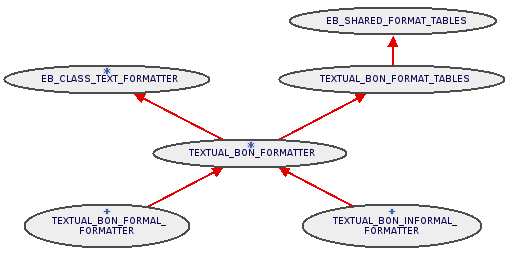
\includegraphics[scale=0.7]{images/textual-bon-formatter.png}
}
\caption{\textsc{textual$\textunderscore$bon$\textunderscore$formatter} inheritance relations.}
\label{fig:textual_bon_formatter}
\end{figure}

\begin{figure}[h]
\centerline{
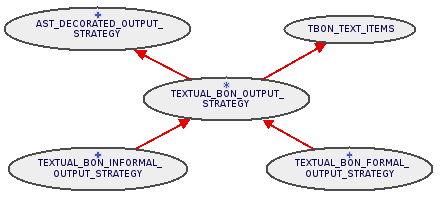
\includegraphics[scale=0.7]{images/bon-extraction-output-strategy.png}
}
\caption{\textsc{textual$\textunderscore$bon$\textunderscore$output$\textunderscore$strategy} inheritance relations.}
\label{fig:bon-extraction-output-strategy}
\end{figure}

\paragraph{}
The output strategies inherits a feature called \textit{process$\_$class$\_$as}. This features purpose is to generate the desired output from a \textsc{class$\_$as}, which is the abstract eiffel syntax representation of a class. In the implementation of the \textsc{bon} tool it does this by instantiated the earlier mentioned meta-object (See figure \ref{fig:bon_extraction_3} on page \pageref{fig:bon_extraction_3}) from the \textsc{class$\_$as} object, which then generated the internal representation. This will be explained in detail in section \ref{tbon_class}.

\paragraph{}
To keep the \textsc{bon} formatters and output strategies both similar, yet distinct at the same time, they both inherit from a shared deferred class, as it can be seen in figures \ref{fig:textual_bon_formatter} and \ref{fig:bon-extraction-output-strategy}. This gives them a polymorphic characteristic, which makes handling these classes easier as it is not always needed know whether you are in formal or informal context at a given point in time. This is not utilized by this project, but is done to make future development more seamless. 

\subsection{BON}
With basis in the \bon{ } grammar (\cite{walden1995}), a series of classes has been created to represent this. These classes are able to store the needed information about the represented grammar object to generate textual \bon. These classes are also responsible for making sure that vital information is present, through \textbf{attached} features and contracts (\textbf{invariants$,$ pre- $and$ postconditions}). Everything knows how to process itself, and itself only. If it contains other elements, such as a class containing features, the class will have a collection of features, and then delegate the ask of processing features to the features itself. Any nested relations are treated like this.

\paragraph{}
This representation of textual \textsc{bon} is based around the \textsc{textual$\_$bon$\_$element} class. From this all classes inherits \textit{process$\_$to$\_$formal$\_$textual$\_$bon} and  \textit{process$\_$to$\_\newline$formal$\_$textual$\_$bon}. These features takes the meta information in the class and formats textual \textsc{bon} based on this information. For some objects that only exist in either formal or informal \bon{ } or are identical in the two, these two features have been renamed to the same (\textit{process$\_$to$\_$textual$\_$bon}).

\paragraph{Completeness}
To give a feeling of working with complete textual \bon{ } other parts than just class chart or class component is generated. In the informal textual \bon{ } view both a system and cluster chart are created. A system chart has the cluster as a collection of clusters, and the cluster then has a collection of clusters and classes. When a system chart is asked to process it will also ask its contained clusters to process, which then will ask its contained classes and clusters to process, in the same way as all other objects in the representation. This is also the case for formal \bon{ } where a cluster component is made.

\paragraph{}
In order to translate the semantics of the indexing clause in Eiffel properly to informal textual \bon{ } a few alterations are made to it. Certain indexing tag names are identified as explanations taken out of the indexing clause and processed under the explanation keyword in textual \bon. This is identified by the \textit{is$\_$explanation$\_$strings} feature in \textsc{tbon$\_$class$\_$chart}. Furthermore an extra indexing clause is added to the informal textual \bon{ }. To identify which cluster a class belongs to a \textit{belongs$\_$to} tag has been added. This is not strictly necessary in this implementation as one cluster is ever only made, however if this was to be expanded to scale to full system, one might want multiple clusters and as such this tag gives the reader better overview.

\paragraph{Inheritance}
To further give the feeling of working with a complete system and to create overview \bon{ } for all descendants of the class in scope is also created. This is done by inspecting the \textit{direct$\_$descendants} feature of the compiled class (\textsc{class$\_$c}). These found classes are then added to the cluster, and are processed through this.

\subsubsection{The meta-object}
\label{tbon_class}
When the output strategy gets the abstract eiffel syntax it needs to create the abstract syntax. As previously mentioned this is done through a meta object. This object is called \textsc{tbon$\_$class}. \textsc{tbon$\_$class} takes a \textsc{class$\_$as} object and instantiates the internal representation of the \bon{}. It does this by inspecting the abstract syntax of the class and giving the needed information to the textual \bon{ } objects.
